```latex
\documentclass{article}

% Required packages for mathematical formulas and symbols
\usepackage{amsmath, amssymb}
% Required packages for creating graphs
\usepackage{tikz}
\usepackage{pgfplots}
\pgfplotsset{compat=1.18} % Ensures compatibility with current pgfplots versions

% Document metadata
\title{Grade 10 Algebra Tutorial: Solving Quadratic Word Problems}
\author{Academic LaTeX Tutor}
\date{\today}

\begin{document}

\maketitle

\begin{abstract}
This document provides a comprehensive tutorial for a Grade 10 algebra problem involving quadratic equations. It includes a detailed problem statement, a step-by-step solution using the quadratic formula and vertex concepts, and an illustrative graph of the quadratic function. The aim is to enhance understanding of quadratic functions in real-world contexts.
\end{abstract}

\section{Introduction}
Quadratic equations are fundamental in algebra and have numerous applications in physics, engineering, economics, and other fields. In Grade 10, students typically learn to solve quadratic equations by factoring, completing the square, and using the quadratic formula. They also learn to interpret the graphs of quadratic functions, which are parabolas, and identify key features such such as the vertex and intercepts. This tutorial will walk through a problem that requires applying these concepts to a practical scenario.

\section{Problem Statement}
A ball is thrown upwards from a platform. Its height $h$ (in meters) above the ground after $t$ seconds is modeled by the quadratic function:
\begin{equation}
h(t) = -5t^2 + 20t + 15
\end{equation}
Answer the following questions based on this model:
\begin{enumerate}
    \item What is the initial height of the ball when it is thrown?
    \item What is the maximum height reached by the ball?
    \item When does the ball hit the ground? (Round your answer to two decimal places.)
\end{enumerate}

\section{Key Concepts}

\subsection{Quadratic Functions}
A quadratic function is a polynomial function of degree two. Its general form is $f(x) = ax^2 + bx + c$, where $a$, $b$, and $c$ are constants and $a \neq 0$. The graph of a quadratic function is a parabola. If $a < 0$, the parabola opens downwards, indicating a maximum point (vertex). If $a > 0$, it opens upwards, indicating a minimum point.

\subsection{Vertex of a Parabola}
For a quadratic function $f(x) = ax^2 + bx + c$, the $x$-coordinate of the vertex (the point where the function reaches its maximum or minimum value) is given by the formula:
\begin{equation}
x = -\frac{b}{2a}
\end{equation}
Once the $x$-coordinate is found, substitute it back into the function to find the corresponding $y$-coordinate (the maximum or minimum value).

\subsection{Roots of a Quadratic Equation (Quadratic Formula)}
The roots (or zeros) of a quadratic equation $ax^2 + bx + c = 0$ are the values of $x$ for which the function equals zero. These can be found using the quadratic formula:
\begin{equation}
x = \frac{-b \pm \sqrt{b^2 - 4ac}}{2a}
\end{equation}
The term $b^2 - 4ac$ is called the discriminant, which determines the nature of the roots.

\section{Worked Examples: Step-by-Step Solution}

Let's solve the problem using the given function $h(t) = -5t^2 + 20t + 15$. Here, $a = -5$, $b = 20$, and $c = 15$.

\begin{enumerate}
    \item \textbf{What is the initial height of the ball when it is thrown?}
    The initial height occurs at time $t=0$ seconds. We substitute $t=0$ into the height function:
    \begin{align*}
    h(0) &= -5(0)^2 + 20(0) + 15 \\
    h(0) &= 0 + 0 + 15 \\
    h(0) &= 15
    \end{align*}
    The initial height of the ball is $15$ meters. This corresponds to the $y$-intercept of the parabola.

    \item \textbf{What is the maximum height reached by the ball?}
    The maximum height occurs at the vertex of the parabola. Since $a = -5$ (which is less than 0), the parabola opens downwards, and the vertex represents a maximum.
    First, find the time $t$ at which the maximum height occurs using the vertex formula $t = -\frac{b}{2a}$:
    \begin{align*}
    t &= -\frac{20}{2(-5)} \\
    t &= -\frac{20}{-10} \\
    t &= 2
    \end{align*}
    The maximum height is reached after $2$ seconds.
    Now, substitute $t=2$ into the height function to find the maximum height:
    \begin{align*}
    h(2) &= -5(2)^2 + 20(2) + 15 \\
    h(2) &= -5(4) + 40 + 15 \\
    h(2) &= -20 + 40 + 15 \\
    h(2) &= 35
    \end{align*}
    The maximum height reached by the ball is $35$ meters.

    \item \textbf{When does the ball hit the ground?}
    The ball hits the ground when its height $h(t)$ is $0$. So, we set the function equal to zero and solve for $t$:
    \begin{equation*}
    -5t^2 + 20t + 15 = 0
    \end{equation*}
    To simplify, we can divide the entire equation by $-5$:
    \begin{equation*}
    t^2 - 4t - 3 = 0
    \end{equation*}
    Now, we use the quadratic formula $t = \frac{-b \pm \sqrt{b^2 - 4ac}}{2a}$, where for this simplified equation, $a=1$, $b=-4$, and $c=-3$:
    \begin{align*}
    t &= \frac{-(-4) \pm \sqrt{(-4)^2 - 4(1)(-3)}}{2(1)} \\
    t &= \frac{4 \pm \sqrt{16 + 12}}{2} \\
    t &= \frac{4 \pm \sqrt{28}}{2} \\
    t &= \frac{4 \pm 2\sqrt{7}}{2} \\
    t &= 2 \pm \sqrt{7}
    \end{align*}
    We have two possible values for $t$:
    \begin{align*}
    t_1 &= 2 + \sqrt{7} \\
    t_2 &= 2 - \sqrt{7}
    \end{align*}
    Numerically, $\sqrt{7} \approx 2.64575$.
    \begin{align*}
    t_1 &\approx 2 + 2.64575 \approx 4.64575 \\
    t_2 &\approx 2 - 2.64575 \approx -0.64575
    \end{align*}
    Since time cannot be negative in this context, we discard $t_2$.
    Therefore, the ball hits the ground approximately $4.65$ seconds after being thrown (rounded to two decimal places).
\end{enumerate}

\section{Illustrative Graph}
The following graph visualizes the height of the ball over time, highlighting the key points calculated in the solution.

\begin{figure}[htbp]
\centering
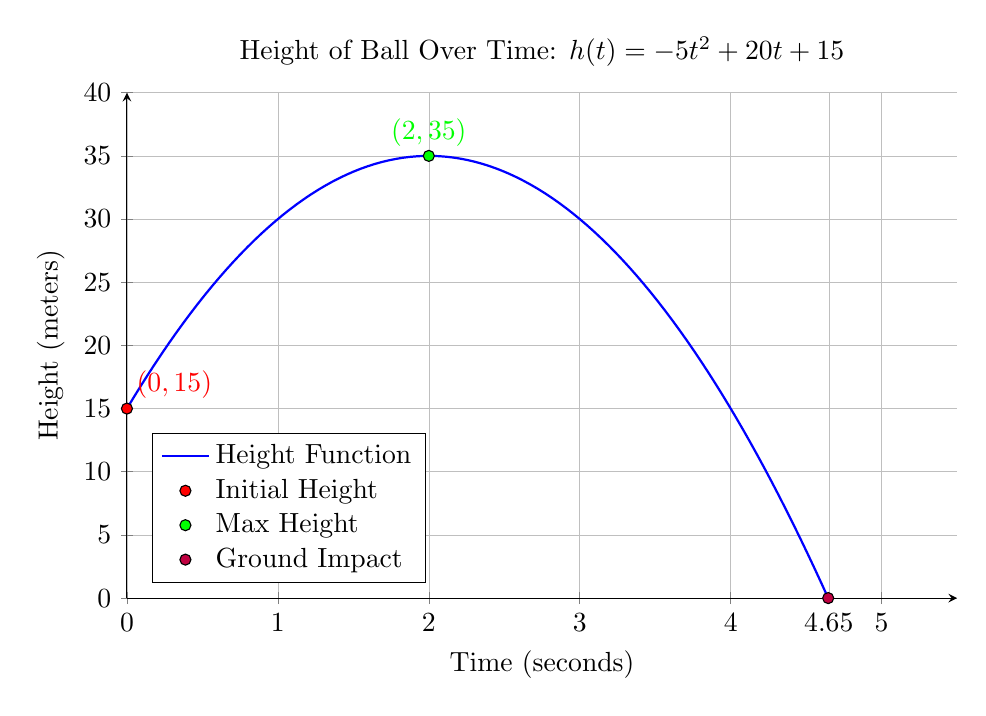
\begin{tikzpicture}
\begin{axis}[
    title={Height of Ball Over Time: $h(t) = -5t^2 + 20t + 15$},
    xlabel={Time (seconds)},
    ylabel={Height (meters)},
    xmin=0, xmax=5.5,
    ymin=0, ymax=40,
    grid=both,
    grid style={line width=.1pt, draw=gray!10},
    major grid style={line width=.2pt,draw=gray!50},
    axis lines=left,
    enlargelimits=false,
    xtick={0,1,2,3,4,4.65,5},
    ytick={0,5,10,15,20,25,30,35,40},
    legend pos=south west,
    legend cell align=left,
    legend entries={Height Function, Initial Height, Max Height, Ground Impact},
    width=\textwidth, % Ensures the graph scales to the text width
    height=8cm % Sets a fixed height for the graph
]
    % Plot the function h(t) = -5t^2 + 20t + 15
    \addplot[domain=0:4.64575, samples=100, blue, thick] {-5*x^2 + 20*x + 15};

    % Mark initial height (t=0, h=15)
    \addplot[only marks, mark=*, mark options={fill=red}] coordinates {(0,15)};
    \node[above right, red] at (axis cs:0,15) {$(0,15)$};

    % Mark maximum height (t=2, h=35)
    \addplot[only marks, mark=*, mark options={fill=green}] coordinates {(2,35)};
    \node[above, green] at (axis cs:2,35) {$(2,35)$};

    % Mark when ball hits the ground (t=4.65, h=0)
    \addplot[only marks, mark=*, mark options={fill=purple}] coordinates {(4.64575,0)};
    \node[below right, purple] at (axis cs:4.64575,0) {$(4.65,0)$};

\end{axis}
\end{tikzpicture}
\caption{Height of a ball over time as modeled by $h(t) = -5t^2 + 20t + 15$.}
\label{fig:ball_height}
\end{figure}

\end{document}
```